%!TEX root = ../thesis.tex
%3-Direct-Spectral-Recovery
% Shift and subtract Method
% Calculation of planet {RV}
% Simulation of spectral recovery
% {RV} difference effect on amplitude of signal simulation
% Chi squared method of model plus stellar at different RVs? technique
% Limitations?
% Future Prospects
% {CRIRES+}, JWST
% Calculation of exposure time required etc?

\chapter{Separating the spectra of faint companions} % Main chapter title
\label{cha:direct_recovery}

There many different techniques to disentangle the spectra of binary objects.
In this chapter we focus on applying a direct subtraction method to near-infrared (\nir{}) spectra of {FGK} stars with Brown Dwarf (BD) companions.
The data used was obtained with the {CRIRES} instrument in 2012 with the purpose to apply this technique specifically.
A level of trust was placed in the quality of the observations, which was misplaced.
We will begin this chapter with the motivation for these specific targets and detail the observations obtained.
We will then present the direct subtraction technique and explore in detail how the observations are insufficient to apply this method, and explore this technique at low RV separations by comparison to simulated results.


Spectral observations of binary systems contain the spectra of both bodies, in proportion to their flux ratio, and Doppler shifted relative to each other due to their orbital motion.
One technique to recover the spectra of the companion is secondary reconstruction through a differential spectrum~\citep{ferluga_separating_1997}.
Spectra from different phases are shifted to the rest frame of the host star and subtracted to mutually cancel out the spectrum of the host star allowing the faint companion spectra to become visible.
Advances in high-resolution and near-infrared (\nir{}) capabilities should enable this technique to be applied to BDs and planet companions, in which smaller {RV} shifts can be resolved and the contrast ratio of the smaller companion is improved.

\section{Spectral Disentangling techniques}

Binary stars through brown dwarfs...
to planets.


Mention the other technique here first.
Then move to the one we tried...




Spectral Disentangling techniques
- PSOAP
- Differencing Fruluga
- Templates?

TODCOR - 2-d from binary analysis~\citep{zucker_study_1994}
\citep{mazeh_detecting_1997}

2-D-cross-correlation?~\citet{piskorz_evidence_2016} seems to have promising technique


\textbf{
See~\citet{kostogryz_spectral_2013} for lots of useful references regarding differential works~\citet{simon_disentangling_1994}}

\citet{rodler_weighing_2012} uses differential of a series of phases to construct a stellar mask for the host to subtract from all measurements.



{\red{}~\citet{kolbl_detection_2015} Use HIRES spectra at 364-799\nm{} (R=60\,000) to determine statistically determine the presence of a faint secondary companion spectra (if any).
They use \textchisquared fitting of the observed spectra against the {SPecMatch} library of observed spectra to find a spectra to best remove the primary star lines,
accounting for dilution and rotational broadening.
They also find that a secondary spectrum with a $\Delta RV$ relative to the host would blend and remain undetectable.
When searching for the secondary they median normalize the spectra into 100K spectra since the difference between stars  <100K different is almost indiscernible in the secondary. The residuals are renormalized and then a \textchisquared fit is again preformed to identify any secondary spectra.
For a low temperature companion (3500K) at a 1\% flux ratio to a 5000-6000\K{} primary star their recovery technique achieves 80\% injection-recovery.}



\section{Motivation}

Motivation section

\textbf{Why this technique and not others.}
- separation of components
- direct imaging (cant separate)


Find direct imaging limitations ---



\textbf{These observations were first taken in an atmospheric window of the \emph{K}-band in order to reduce the absorption introduced by the atmosphere~\citep{barnes_hd_2008}.
}
\section{Motivation and target selection}
\label{sec:target_motivation}
The work of~\citet{sahlmann_search_2011} identified several candidate brown dwarf companions of FGK stars with \(\rm M_2 \sin{i}\) values > 10~\Mjup{}.
Seven candidates from~\citet{sahlmann_search_2011}, which were visible in Period 89 (2012), were selected for further observation in order to identify their stellar nature.
That is, to refine the mass of the companions to distinguish if their companion is a large giant planet (M$\apprle13$\Mjup), a Brown dwarf (13$\apprle $M$\apprle80$\Mjup), or a low-mass star (M$\apprge80$\Mjup).

The spectral differential approach was chosen with the goal to constrain the companion masses while minimizing the observational time required to observe.
It was deemed that it should be possible to obtain a detection of a companion at 1\% contrast ratio with an exposure time of around 20 minutes.
Two observations at ``clearly separate RVs'' were requested to constrain each target.
Observations were preformed without telluric standard star observations to avoid the wasted observing time, choosing to instead rely on synthetic model correction (see \cref{sec:telluric_correction}).
The \textit{K}-band was chosen to achieve a high contrast relative to the host star, detected in the extreme V-K colour indexes (>7.8).

The list target host stars are presented in \cref{tab:star_params} along with their stellar parameters, while the companion orbital parameters are provided in \cref{tab:orbitparams}.

We note that the orbital parameters of some targets have been refined in the literature since the observations took place.
For example three candidates have had their masses refined in recent works.
The companion to {HD\,211847} was determined to be a low mass star with \(\rm M_2=155~\)\Mjup{}~\citep{moutou_eccentricity_2017}, while the companion to {HD\,4747} was found to have a mass of \(\rm M_2=60~\)\Mjup{}~\citep{crepp_trends_2016}.
The two companions of {HD\,202206} (B and c) were found to have masses of \(\rm M_B =93.6\)~\Mjup{} and \(\rm M_c = 17.9\)~\Mjup{}, respectively, classifying {HD\,202206}c as a ``circumbinary brown dwarf''~\citep{benedict_hd_2017}.
These three companions with recently refined masses (along with {HD\,30501}) create a good set of benchmarks to compare any results from the techniques developed here, and show that the masses of these targets do span the BD to low mass star range.
All target companions except {HD\,162020} (P=8.4 days) are in (very) long period orbits (P=0.7--38 years) with masses (or \Mtwosini{}) greater than 10~\Mjup{}.

%!TEX root = ../../thesis.tex

%% Table of stellar parameters
\begin{table*}
    \centering
    \begin{threeparttable}[b]
        \caption{Stellar parameters of the host stars.
V is the apparent magnitude taken from {SIMBAD}~\citep{wenger_simbad_2000}. {Distances were calculated from the GAIA DR2 parallax measurements.}}
        \begin{tabular}{l c c r@{$~\pm~$}l r@{$~\pm~$}l r@{$~\pm~$}l r@{$~\pm~$}l c c c}
            \toprule
            Star & SpT & V & \multicolumn{2}{c}{\(T_{\textrm{eff}}\) (K)} & \multicolumn{2}{c}{logg (cm s\(^{-2} \))} & \multicolumn{2}{c}{[Fe/H]} & \multicolumn{2}{c}{\(M_1\) (\textrm{M}\(_{\odot} \))} & Age (Gyr) & d (pc) & Reference\\
            \midrule
            {HD 4747} & K0V & 7.15 & 5316 & 50 & 4.48 & 0.10 & $-$0.21 & 0.05 & 0.81 & 0.02 & $3.3 \pm 2.3$ & $18.80 \pm 0.04$ & 1, 2, 3, 8 \\
            {HD 162020} & K3V & 9.12 & 4723 & 71 & 4.31 & 0.18 & $-$0.10 & 0.03 & 0.74 & 0.07 & $3.1 \pm 2.7$ & $30.85 \pm 0.06$ & 4, 5, 6, 8 \\
            {HD 167665} & F9V & 6.40 & 6224 & 50 & 4.44 & 0.10 & 0.05 & 0.06 & 1.14 & 0.03 & 0.7 -- 3.6 & $ 31.24 \pm 0.06$ & 1, 8 \\
            {HD 168443} & G6V & 6.92 & 5617 & 35 & 4.22 & 0.05 & 0.06 & 0.05 & 1.01 & 0.07 & $10.0 \pm 0.3$ & $39.67 \pm 0.12$ & 5, 6, 8 \\
            {HD 202206} & G6V & 8.07 & 5757 & 25 & 4.47 & 0.03 & 0.29 & 0.02 & 1.04 & 0.07 & $2.9 \pm 1.0$ & $46.03 \pm 0.14$ & 5, 7, 8 \\
            {HD 211847} & G5V & 8.62 & 5715 & 24 & 4.49 & 0.05 & $-$0.08 & 0.02 & 0.92 & 0.07 & 0.1 -- 6.0 & $48.81 \pm 0.13 $ & 1, 2, 4, 8 \\
            {HD 30501} & K2V & 7.59 & 5223 & 50 & 4.56 & 0.10 & 0.06 & 0.06 & 0.81 & 0.02 & 0.8 -- 7.0 & $20.37 \pm 0.01$ & 1, 4, 8 \\
            \bottomrule
        \end{tabular} \label{tab:starparams}
        \begin{tablenotes}
           \item[] References: (1)~\citet{sahlmann_search_2011}; (2)~\citet{santos_spectroscopic_2005}; (3)~\citet{crepp_trends_2016}; (4)~\citet{tsantaki_deriving_2013}; (5)~\cite{bonfanti_age_2016}; (6)~\citet{santos_spectroscopic_2004}; (7)~\citet{sousa_spectroscopic_2008}; (8)~\citet{collaboration_gaia_2018};
        \end{tablenotes}
    \end{threeparttable}
\end{table*}

%!TEX root = ../../thesis.tex
% Table of orbit parameters

\todo{Rotate orbital parameter table.}
\begin{table*}
    \centering
    \caption[Orbital parameters of companions.]{Orbital parameters for the BD companions obtained from the literature.}
    \begin{tabular}{l c r@{$ \,\pm\, $}l r@{$ \,\pm\, $}l r@{$ \,\pm\, $}l r@{$ \,\pm\, $}l r@{$ \,\pm\, $}l cc c c}
        \toprule
        Object  & \(\gamma\) & \multicolumn{2}{c}{Period} & \multicolumn{2}{c}{\(e\)} & \multicolumn{2}{c}{\(\kone\)} &  \multicolumn{2}{c}{\(T_{0}\)} & \multicolumn{2}{c}{\(\omega\)} & \Mtwosini{} & \(\mtwo\) & Ref.\\
        & (\kmps{}) & \multicolumn{2}{c}{(day)} & \multicolumn{2}{c}{} & \multicolumn{2}{c}{(\mps{})} & \multicolumn{2}{c}{(JD-2,450,000)} &  \multicolumn{2}{c}{(deg) } & (\Mjup{}) & (\Mjup{}) & \\
        \midrule
        \object{HD 4747}  & $0.215 \pm 11 $    &  13\,826.2  &  314.1   &  0.740 & 0.002 & 755.3   &  12 & 463.1  &  7.3    & 269.1 &  0.6   &  39.6    & 60.2  & 1 \\
        \object{HD 162020}   & $-27.328\pm0.002$ &  8.42819  &  $6e^{-5}$   &  0.277 & 0.002   & 1\,813    &  4   & 1\,990.68   &  0.01  & 28.4   &  0.2   & 14.4     &     -    & 2 \\
        \object{HD 167665}   & $8.003 \pm 0.008$    & 4\,451.8 & 27.6     & 0.340 & 0.005  & 609.5   &  3.3     & 6\,987.6     &  29     & $-$134.3 & 0.9     & 50.3    &     -   & 3 \\
        \object{HD 168443}b  & $-0.047\pm0.552$     & 58.1124 & $4e^{-4}$ & 0.529 & 0.001   & 475.13 & 0.9 & 5\,626.20  &  0.02   & 172.9 & 0.1     & 7.7 &     -   & 4 \\
        \object{HD 168443}c  & $-0.047\pm0.552$ & 1\,749.83 & 0.57 & 0.211 & 0.002  & 297.7  & 0.6 & 5\,521.3     &  2.2     & 64.9  & 0.5     & 17.1    &     -     & 4 \\
        \object{HD 202206}B & 14.721   & 256.33  &  0.02    & 0.432 & 0.001   & 567     &  1  & 2\,176.14    &  0.12   & 161.9     & 0.2 & 17.4    & $93.2\pm7.3$   & 5, 6\\
        \object{HD 202206}c & 14.721   & 1\,260 &  11 & 0.22 & 0.03  & 41   & 1 & 3\,103     & 452    & 280   & 4   & 2.3 & $17.9\pm2.9$  & 5, 6\\
        \object{HD 211847} & 6.689\tablefootmark{a} & 7\,929.4 & 2\,500 & 0.685 & 0.068    & 291.4   & 12.2   & 12\,030.1    & 2\,500   & 159.2     & 2.0     & 19.2  & 155 & 3, 7\\
        \object{HD 30501}   & $23.710\pm0.028$    & 2\,073.6 & 3.0    & 0.741 & 0.004 & 1\,703.1 & 26.0   & 3\,851.5     & 3.0     & 70.4     & 0.7     & 62.3   & 89.6     & 3  \\
        \bottomrule
    \end{tabular}\label{tab:orbitparams}
    \tablebib{
             (1)~\citet{crepp_trends_2016}; (2)~\citet{udry_coralie_2002}; (3)~\citet{sahlmann_search_2011};
             (4)~\citet{pilyavsky_search_2011}; (5)~\citet{correia_coralie_2005}; (6)~\citet{benedict_hd_2017}; (7)~\citet{moutou_eccentricity_2017}
    }
    \tablefoot{
    \tablefoottext{a}{fixed}
    }
\end{table*}
\todo{Needs rotation}

\subsection{The Data}

\subsection{CRIRES data}
\label{subsec:CRIRES}
Observations were performed with the {CRIRES} instrument~\citep{kaeufl_crires_2004} configured to observe a narrow wavelength domain of the \emph{K}-band between 2\,120--2\,160\nm{}.
The slit width of \(0.4^{\prime\prime}\) resulted in an instrumental resolving power of \(\R=50\,000\)\footnote{The rule of thumb resolution for {CRIRES} is \(100\,000\times \frac{0.2^{\prime\prime}}{\textrm{slit width}}\) with the slit width in arcseconds}.
No adaptive optics were used to ensure that the entrance slit was entirely covered by each target.
This is to prevent strong slit illumination variations that could change the shape of spectral lines.

The observations were performed in service mode during Period 89 with run {ID.~089.C-0977(A)} between April and August 2012.
A single observation is composed of eight individual spectra with an integration time of 180\si{\second} each, observed in the {ABBAABBA} nod cycle pattern to obtain a high signal-to-noise (>100) when combined.
The list of observations obtained with {CRIRES} are provided in \cref{tab:observations}.

There is a slight inconsistency with the some of the observations, taken in service mode.
For instance {HD\,202206} has two observations taken with the {Ks} filter, while one is taken with the {J} filter.
There is also the last observation of {HD\,30501} taken with a different filter that the others.
The phase two observing proposal documents were unable to obtained to access determine if these odd filters were requested like this or if it was an observational mistake.

There is also an inconsistency with the ordering of the observations again with the target {HD\,202206}.
The observation that was performed first in time is labelled with the observation name of {HD\,202206-3} in the fits header file, while the second and third observations are labelled -1 and -2 respectively.

There could be two possible reasons for the single observation of {HD\,4747}.
One is that only one observation was requested due to the very long orbital period of the target, although this would not fulfil the science goal.
The other more likely reason is that these observations were preformed in service mode as a filler program and in the end there was no time to observe a second observation of {HD\,4747}.

\textbf{Is there a reason for the two different filters?}

%!TEX root = ../../nir_companions.tex
\todo{rotate table?}
% Table of observations
\begin{table*}
    \small
    \centering
    \begin{threeparttable}[b]

        \caption{Details about the each {CRIRES} observation. The number of artefacts removed in \sref{subsubsec:reductionartefacts} as well as the {SNR} of the combined spectra is provided. The last three columns are the calculated {RV} of both host and largest companion, from the orbital solution, as well as the {RV} difference between the two components.}
        %\begin{tabular}{l c c c c cl cl r@{.}l r@{.}l r@{.}l}
        \begin{tabular}{l c c c c c c | r@{.}l r@{.}l r@{.}l}
            \toprule
            Object & Obs.& Start date  & Filter & Airmass  & Artefacts & {SNR} & \multicolumn{2}{c}{\(RV_1\)} & \multicolumn{2}{c}{\(RV_2\)} & \multicolumn{2}{c}{\(rv_2\)}  \\  % & \(Date \)
            &  \#   & (yyyy-mm-dd hh:mm:ss)  &  & (at start) & {/ 32} & & \multicolumn{2}{c}{\kmps{}} & \multicolumn{2}{c}{\kmps{}} & \multicolumn{2}{c}{\kmps{}}\\ % data ref    % & (JD\(^{\star} \))
            \midrule
            {HD 4747}   & 1 & 2012-07-06 07:36:06 & Ks            & 1.25     & 7 & 340 & $-$0 & 219 & $-$0  & 154 & 0&065 \\ %-1   & 2456\,114.81674
            {HD 162020} & 1 & 2012-07-04 06:23:22 & Ks      & 1.30  & 2 & 127 & $-$28  & 760 & 50 & 785\tnote{a}  & 79&545\tnote{a} \\ %-1   & 2456\,112.76624
            {HD 162020} & 2 & 2012-07-04 06:57:48 & Ks      & 1.44   & 2 & 128 & $-$28  & 717 & 48 & 440\tnote{a} & 77&157\tnote{a} \\ %-2   & 2456\,112.79015
            {HD 167665} & 1 & 2012-07-28 05:00:53 & Hx5e-2  & 1.24  & 7 & 371 & 7      & 581 & 18 & 024\tnote{a} & 10&443\tnote{a} \\ %-1a  & 2456\,136.70895
            {HD 167665} & 2 & 2012-07-28 05:37:27 & Hx5e-2  & 1.39   & 4 & 374 & 7      & 581 & 18 & 025\tnote{a}  & 10&444\tnote{a} \\ %-1b  & 2456\,136.73434
            {HD 167665} & 3 & 2012-08-05 02:54:03 & Hx5e-2  & 1.04   & 4 & 358 & 7      & 575 & 18 & 163\tnote{a} & 10&588\tnote{a} \\ %-2   & 2456\,144.62087
            {HD 168443} & 1 & 2012-08-05 04:29:32 & Ks      & 1.31  & 2& 192 & $-$0   & 121 & 50 & 932\tnote{a,b}  & 51&053\tnote{a,b} \\ %-1   & 2456\,144.68718
            {HD 168443} & 2 & 2012-08-05 04:58:50 & Ks      & 1.47  & 4 & 190 & $-$0   & 121 & 51 & 189 \tnote{a,b} & 51&310\tnote{a,b} \\ %-2   & 2456\,144.70753
            {HD 202206} & 1 & 2012-07-12 06:54:44 & Ks      & 1.01  & 3& 189 & 14   & 843 & 12 & 992\tnote{b}  & -1&851 \\ %-1   & 2456\,120.78801
            {HD 202206} & 2 & 2012-07-13 05:41:40 & J          & 1.01    & 3 & 209 & 14   & 837 & 13 & 065\tnote{b}  & -1&772 \\ %-2   & 2456\,121.73727
            {HD 202206} & 3 & 2012-07-11 08:29:55 & Ks      & 1.15 & 4& 180 & 14   & 849 & 12 & 920\tnote{b}  & -1&929 \\ %-3   & 2456\,119.85411
            {HD 211847} & 1 & 2012-07-06 07:02:57 & Ks      & 1.07  & 4& 272 & 6     & 613 & 7   & 171 & 0& 558\\ %-1   & 2456\,114.79372
            {HD 211847} & 2 & 2012-07-13 06:54:37 & Ks      & 1.05  & 5& 283 & 6     & 614 & 7   & 167 & 0&553 \\ %-2   & 2456\,121.78793
            {HD 30501}  & 1 & 2012-04-07 00:08:29 & Hx5e-2   & 1.60   & 3& 217 & 22   &  372 & 36 & 377 & 14&005 \\ %-1   & 2456\,024.50590
            {HD 30501}  & 2 & 2012-08-01 09:17:30 & Hx5e-2 & 1.42  & 10& 212 & 22   & 505 & 35  & 120 & 12&615 \\ %-2a  & 2456\,140.88716
            {HD 30501}  & 3 & 2012-08-02 08:47:30 & Hx5e-2   & 1.53   & 8& 237 & 22   & 507 &  35 & 102 & 12&595 \\ %-3   & 2456\,141.86633
            {HD 30501}  & 4 & 2012-08-06 09:42:07 & Ks       & 1.28   & 7& 235& 22   & 514 & 35 & 031 & 12&517 \\ %-2b  & 2456\,145.90426
            \bottomrule
            & & & &
        \end{tabular}\label{tab:observations}
        \begin{tablenotes}
            \item  [a]{Maximum {RV} given \mtwosini{} only.}
            \item  [b]{Largest mass companion only.}
        \end{tablenotes}
    \end{threeparttable}
\end{table*}



\textbf{The filters...using the {Ks} and the {Hx5e-2} filters, Why use the different filters???}

All observations were reduced using the {DRACS} pipeline with the artefact corrections applied (see \cref{subsec:pipeline-selection}).
Each observation was wavelength calibrated and corrected for telluric lines then corrected for the barycentric RV following  \cref{subsec:wavecalib,subsec:telluric_correction_application,subsec:barycentriccorrection}.


\subsection{Calculations using observed times}
\todo{I am not sure if this is the best location for this section.}
{\red{}
Before the differential subtraction method is presented, calculations can be preformed to estimate the RV of both components in each observations and the likely separation between the companions between observations.
The time of each observation is combined with the orbital parameters from \cref{tab:orbitparams} to calculate the RV of the host star (\({RV}_{1}\) in \cref{tab:observations}) using \textbf{EQUATION XX}.
For the companion, the mass (\Mtwo or \Mtwosini{}) is used alongside the stellar mass from \cref{tab:star_params} to calculate the RV of the companion using \todo{~equations for companion rv with the masses still included, include 180 degree angle phase change also}{\textbf{cref{}}}.
This is given as \({RV}_{2}\) in \cref{tab:observations}.
The estimated difference in RV between the host and companion for each observation is also computed as \({rv}_{2} = {RV}_{2}-{RV}_{1}\) although it will not be used until \cref{cha:model_comparison}.

For these observations the maximum estimated RV separation between the two companion spectra in  \(\Delta RV\) is calculated following \cref{eqn:companion_difference} and provided in \cref{tab:estimated_rv}.
This table also contains the estimated semi-major RV amplitude for the companion \(K_2\) and the phase coverage from the observations.
The phase coverage is the fraction of the orbit covered between the observations for each target.
For {HD\,4747} the \(\Delta RV\) and phase coverage values are missing due to the single observation.
}

%!TEX root = ../../thesis.tex
\begin{table*}
    %\small
    \centering
    \begin{threeparttable}[b]
        \caption[Semi-amplitude and RV separation of companions.]{Estimated orbital semi-amplitude and {RV} separation of the companions, given the companion mass (\Mtwo{} or \Mtwosini{}) from \cref{tab:orbitparams} and observation times from \cref{tab:observations}.}
        \begin{tabular}{l c c c c c c}%[hb]
            \toprule
             & Estimated & Estimated & & \\  % 2017
             Companion & \Ktwo{} & |\(\Delta {RV}\)| & Phase coverage\\
             & (\kmps{}) & (\mps{}) & (\%)\\
             \midrule
             {HD 4747} & -10.65 & -- & --\\  % 2017
             {HD 162020} & -98.92\tnote{a} & 2388 & 0.28\\  %
             {HD 167665} & -14.47\tnote{a} & 145 & 0.18\\  %  -- \(2\times10^{-5} \)  best case based on age rage.
             {HD 168443b} & -64.65\tnote{a} & 258 & 0.035\\
             {HD 168443c} & -18.05\tnote{a} & <1 & 0.001\\  %(c)
             {HD 202206}B & -6.79 & 78 & 0.74\\  %(B)   % May2017
             {HD 202206}c & -2.50 & <1 & 0.15\\  %(B)   % May2017
             {HD 211847}B & -1.85 & 5 & 0.09\\  %B % 2017
             {HD 30501} & -16.12 & 1410 & 5.8\\
             \bottomrule
         \end{tabular}\label{tab:estimated_rv}
         \begin{tablenotes}
            \item[a] {Maximum \Ktwo{} only given \Mtwosini.}
         \end{tablenotes}
    \end{threeparttable}
\end{table*}

%%!TEX root = ../thesis.tex
\todo{check hspace spacing}
\begin{table*}
    %\tiny
    \small
    \centering
    \caption[Estimated flux ratios and semi-amplitude of the companion.]{Estimated flux ratios and semi-amplitude of the companion given the companion \(\textrm{M}_{2}/\textrm{M}_{2} \sin{i}\) from \cref{tab:orbitparams}.
    The flux ratio \(F_{2}/F_{1} \) is calculated using the \emph{K}-band magnitude difference of the host star to the Baraffe evolutionary model magnitude for the companion mass.
    The model ages used are those closest to host age value in \cref{tab:star_params}.
    The noise ratio is calculated via \(N_{2}/N_{1} = \sqrt{2} \times\sqrt{F_{1}/F_{2}}\).
    The orbital properties are calculated using the orbital parameters given above along with the times of observations in \cref{tab:observations}.}
    \begin{tabular}{l c c c c c c c c}
        \toprule
        &  Estimated  & Estimated &  Estimated & Estimated &  &    \\  % 2017
        Host           & \(\rm F_{2}/F_{1} \)   & \(\rm N_{2}/N_{1} \) (noise ratio) & \(\rm K_2\) &   \(\Delta {RV}\) & Phase coverage \\
        & \emph{K}-band     & & (\kmps{}) & (\mps{}) & (\%) \\
        \midrule
        \object{HD 4747}        & \(3\times10^{-4} \)   & 76 &  -10.65 & -  &  -  \\  % 2017
        \object{HD 162020}   & \(7\times10^{-7} \)   & 1\,615  &  -98.92\tablefootmark{a} &  2\,344.24     & 0.28\hspace{4em} \\  %
        \object{HD 167665}    & \(2\times10^{-4} \)   &  105    &  -14.47\tablefootmark{a}   &   138.45     & 0.18\hspace{4em}\\  %  -- \(2\times10^{-5} \)  best case based on age rage.
        \object{HD 168443b} & \(1\times10^{-16} \)  &    \(1\times10^{8} \)   &  -64.65\tablefootmark{a} &   257.16   & 0.035 \\
        \object{HD 168443c} &  \(1\times10^{-11} \)  &   \(4\times10^{5} \)     &  -18.05\tablefootmark{a}  &   0.95   &  0.001 \\  %(c)
        \object{HD 202206}B  & \(8\times10^{-7} \)  &   1\,586 &  -6.79 & 145.17   & 0.74\hspace{3em}   \\  %(B)   % May2017
        \object{HD 202206}c  &  \(5\times10^{-15}\)   &     \(2\times10^{7} \) &   -2.50     &   0.67     &  0.15\hspace{3em} \\  %(B)   % May2017
        \object{HD 211847}B  &  0.01 &  14   & $-$1.85 & 3.88   & 0.09\hspace{3em} \\  %B % 2017
        \object{HD 30501}      &  0.002  &  27  &  -16.12    &  1\,346.46      & 5.8\hspace{4em}\\
        \bottomrule
    \end{tabular}\\
    \tablefoot{
        \tablefoottext{a}{Maximum \(K_2\) only given \(M_2 \sin{i}\)}
    }
    \label{tab:flux_table}
\end{table*}
 % This is the old table.

The full orbital solution for the components along with the times of observations are provided later in \cref{sec:orbtial_diagrams}.


\section{Direct Subtraction Method}
\label{sec:direct-subtraction}
Here the direct subtraction method used is presented, which is similar to previous works~\citep{ferluga_separating_1997, kostogryz_spectral_2013}.
Assuming that the instrumental profile and atmospheric absorption are dealt with appropriately the spectra of the observed targets are assumed to be composed of two spectral components:
a bright host star blended with the spectrum of a faint companion.
The spectrum received from the host-companion pair is given by the superposition of two spectral components (\(J_{1}\), \(J_{2}\)):
\begin{equation}
\textrm{I}(\lambda) = \textrm{J}_{1}(\lambda - v_{1}) + \textrm{J}_{2}(\lambda - v_{2}),
\end{equation}
where the subscripts 1 and 2 indicate the spectrum of the host and companion respectively, \(\lambda\) represents the wavelength of the spectra and \(\lambda-v\) represents the Doppler shift \(\lambda(1-v/c)\) by a velocity \(v\).

This can be shifted into the rest frame of the host star by applying the shift \(v_1\):
\begin{equation}
\textrm{I}(\lambda + v_{1}) = \textrm{J}_{1}(\lambda) + \textrm{J}_{2}(\lambda - v_{2} + v_{1}).
\end{equation}

To analyse \(J_2\), the spectral component of interest, the component from the host needs to be carefully removed.
If two observations of the same target are observed, denoted with subscripts \(a\) and \(b\), there will be relative motion between the components due to the orbit.
Assuming that the stellar spectra do not change over time (\(J_{1a} = J_{2a}\)) and each spectrum can be individually Doppler shifted to the rest frame of the host star \(J_1{\lambda}\), then the spectrum of the host star (\(\textrm{J}_{1}\)) can be removed though subtraction of the two observations.
Mutually cancelling the host component leaves two components of the companion subtracted from each other, with a relative Doppler shift between them.
\begin{align}
S(\lambda) &= \textrm{I}_{a}(\lambda + v_{1a}) - \textrm{I}_{b}(\lambda + v_{1b}) \nonumber \\
&= (\textrm{J}_{1a} + \textrm{J}_{2a}(\lambda - v_{2a} + v_{1a})) - (\textrm{J}_{2b} +\textrm{J}_{2b}(\lambda - v_{2b} + v_{1b})) \nonumber \\
&= \textrm{J}_{2a}(\lambda - v_{2a} + v_{1a}) - \textrm{J}_{2b}(\lambda - v_{2b} + v_{1b}) \nonumber \\
% &= \textrm{J}_{2}(\lambda - v_{2a}) - \textrm{J}_{2}(\lambda - v_{2b} - v_{1a} + v_{1b}) \nonumber \\
S(\lambda + v_{2a}-v_{1a}) &= \textrm{J}_{2a}(\lambda) - \textrm{J}_{2b}(\lambda - v_{2b} - v_{1a} + v_{1b} + v_{2a})\\
S(\lambda') &= \textrm{J}_{2a}(\lambda) - \textrm{J}_{2b}(\lambda - \Delta {RV}_2) \label{eqn:sprofile}
\end{align}
where,
\begin{equation}
\Delta {RV}_2 = v_{1a} - v_{1b} - v_{2a} + v_{2b} \label{eqn:companion_difference}
\end{equation}
is the {RV} difference between the two companion spectral components when the host components are mutually subtracted,
and \(\lambda' = \lambda + v_{2a}-v_{1a}\).

The resulting differential spectra \(S({\lambda'})\), dubbed \emph{s-profile} by~\citet{ferluga_separating_1997}, is composed of just the companion spectra, shifted and subtracted from itself.

\citet{ferluga_separating_1997} provide an analytical form for the \emph{s-profile} given a single Gaussian line of the form
$J(\lambda) = 1- D \cdot\exp^{{-\pi {(\lambda - \lambda_0)}^2} / {{W}^{2}}}$:
\begin{equation}
    S(\lambda) = 2 D\cdot\exp^{{-\pi {D}^{2} [{(\lambda - \lambda_0)}^{2} +{(k/2)}^{2}]}/{{W}^{2}}} \cdot \sinh{\frac{\pi {D}^{2}(\lambda-\lambda_0)k}{{W}^{2}}},\label{eqn:sprofile_gaussain}
\end{equation}
where $\lambda_0$, $D$, and $W$ are the central wavelength, depth and equivalent width of the Gaussian line, and $k=\Delta {RV}_2 $ is the shift between the two companion spectra.


From binary dynamics~\citep[e.g.][]{murray_keplerian_2010} the {RV} amplitudes of the host and companion are related through the mass ratio, \(q\), while having an opposite sign\footnote{The opposite sign arises from a \(180^\circ\) difference in the angle of periapsis, \(\omega\), for the companion.}:
\begin{align}
v_{2} &= -q * v_{1} \label{eqn:q_relation}
\end{align}
\todo{put in advanced concepts chapter???}
\todo{this ignores $\gamma$}
We can simplify \cref{eqn:companion_difference} by expressing it in terms of the mass ratio and host {RV} only:
\begin{align}
\Delta RV_2 &= q v_{1a} - q v_{1b} + v_{1a} - v_{1b} \nonumber \\
&= (1 + q)(v_{1a} - v_{1b}). \label{eqn:companion_difference_simplified}
\end{align}

If the \(\Delta {RV}_2\) between the companion spectra is able to be derived from the s-profile~\citep[see][]{ferluga_separating_1997} then the mass ratio of the system, \(q\), can be determined, thereby constraining the mass of the companion.

The values \(v_{1a}\) and \(v_{1b}\) are radial velocity of the host components.
The host's RV are calculated using the \cref{eqn:rv_equation} with the orbital parameters from the literature and provided in \cref{tab:orbitparams}.
These are used to shift each spectrum into the rest frame of the host star to mutually cancel the host's spectrum.
These components can also be determined directly from the spectrum by cross-correlating the observed spectrum with a stellar template of the host and gave results in reasonable agreement.
There should be checks for consistency between \(v_{1a}\), \(v_{1b}\) and how well the host component is removed in the s-profile.

\textbf{If v1a and v1b are incorrect what will happen to q?}

{\red{} put elsewhere: \cref{eqn:q_relation} was used to calculate the expected companion {RV} for each observation in \cref{tab:observations}.}

Example simulations?
\missingfigure{simulated example of combined binary spectra, and the subtraction, with a clear companion visible }

\textbf{\citet{kostogryz_spectral_2013} use a very similar method, choosing two observations from the extrema.
They also preform a number of simulations regarding observing CRIRES spectra with different brown dwarfs.
Figure out the flux ratio limit they get too???}

\subsection{Results of spectral differential analysis}
\label{subsec:differential_results}

We applied the spectral differential procedure outlined above on the wavelength-calibrated and telluric-corrected {CRIRES} observations.
The spectra were first Doppler shifted to the rest frame velocity of the system by applying a shift of \(-\gamma\).
The differential subtraction method was then applied by shifting each spectra so that the host lines were at rest and then subtracting one from the other as described above.

It is necessary to have a consistent instrumental setup~\citep{ferluga_separating_1997}, to avoid introducing extra instrumental effects (e.g.\ slit-width and/or filters) into the spectral differentials and to always observe the same wavelength range and maximize the information to be extracted.
In our case, the second observation of {HD\,202206} and fourth of {HD\,30501} were taken with different filters compared to the other observations.
Therefore, these two observations could not be used for this differential analysis.
As noted in~\citet{hadrava_disentangling_2009}, any spectral differences in the filters would add extra unknown signal/noise making it harder to disentangle the faint spectral differences.

We performed the differential analysis for all targets but only show our most favourable case here, {HD\,30501}, because it is the second largest companion in our sample at 90~\Mjup{} and also has the second largest {RV} separation between observations.
The differential spectra recovered for {HD\,30501} is shown at the bottom panel of \cref{fig:spectral_example}.
The presence of deep (\(>4\%\)) stellar and telluric lines in the original spectrum is shaded by the blue and green regions respectively.
This indicates that the features of the differential spectrum near these shaded regions are likely due to imperfect telluric correction and host mutual cancellation.

The mutual cancellation of the stellar host works well for the \(\sim40\%\) deep line near 2\,117\nm{}, being completely removed, but it does not do so well for the smaller \(\sim10\%\) deep line around 2\,121.5\nm{}.
The residual for the large \(\sim40\%\) deep telluric line near 2\,118.5\nm{} is quite prominent.
There is also a wider residual due to three neighbouring lines \(\sim10\%\) deep around 2\,120\nm{} which cause features in the differential spectrum.
One possible explanation is that the continuum normalization near 2\,120\nm{} was influenced by this grouping of lines.

To understand the observed differential signal we simulated a differential spectrum of {HD\,30501} using a synthetic {PHOENIX-ACES} spectra with parameters \(\teff{}=2\,500\)\K{}, \logg{}=5.0, and \feh{}=0.0, with a {RV} offset estimated from the observation times.
These parameters represent an estimated companion \(\teff{}\) with the metallicity and \logg{} similar to the host (closest grid model).
The model spectra were convolved to \(\R=50\,000\), continuum normalized and scaled by the estimated flux ratio of the companion.
We do not include any synthetic host or telluric spectra and as such simulate the differential result of a ``perfect'' host cancellation with no telluric contamination present.
This is the ideal-case scenario, and we stress that it is impossible to simulate the effect of improper telluric correction in a meaningful way.
When comparing the simulated and observed differential in the bottom panel of \cref{fig:spectral_example}, there is a striking amplitude difference.
The orange-dashed line of the simulated differential spectrum amplitude is of a much smaller scale than the observed differential.
This demonstrates that the amplitude of the differential signal we are trying to detect is much smaller than the residuals created by this differential technique.

The amplitude of the differential signal is lower than we expected due to the very low \(\Delta {RV}\) between the observation pairs.
The maximum \(\Delta {RV}\) between observation pairs, for the observations investigated in this work, are provided in \cref{tab:estimated_rv}.
{\red{} There is no \(\Delta {RV}\) for {HD\,4747} as there was only a single observation.
We also provide the phase coverage for our targets.
We calculate this as the ratio of time between the observed pairs and the orbital period, and show that the fraction of the orbit covered is very small; all except one covering less than 1\% of the orbit.}\todo{this is duplicated }

In our best case, {HD\,30501}, the \(\Delta {RV}\) of the companion between observations is 1.41\kmps{}.
For comparison, a single Gaussian absorption line, to be shifted by \(\Delta\lambda = {\fwhm}\) would need a \(\Delta {RV}\) of \(v_{\fwhm} = c/\R =~\sim6\)\kmps{}.
Since the \(\Delta {RV}\) are shifted by a smaller value than the {\fwhm}, the spectral lines of the reconstruction mutually cancel themselves, diminishing the amplitude of the differential signal significantly.
As the companion spectra are already faint (with a flux ratio at the percent level) the differential signal is not detectable within these observations and noise level.

When the \(\Delta {RV}\) of the companion is smaller than the {\fwhm} of a line there is a mutual subtraction of the companion spectra, diminishing the detected amplitude of the differential signal, and removing the ability to detect the companions using this method.
Observations need to be spaced further apart in time/phase to achieve a larger \(\Delta {RV}\) separation and increase the amplitude of the differential.
Of course once there is a separation there will be complex interactions between neighbouring lines that need to be accounted for.

\begin{figure}
    \centering
    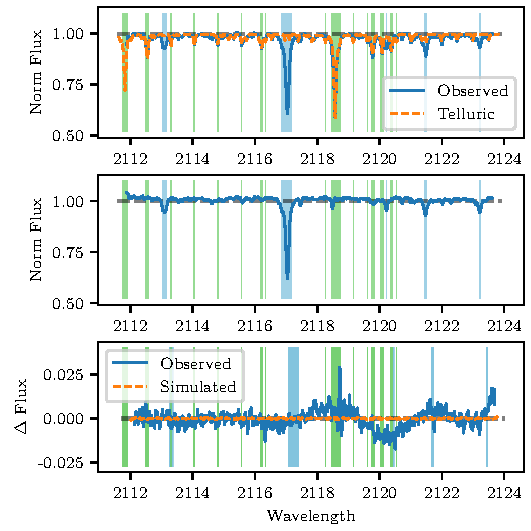
\includegraphics[width=0.8\hsize]{figures/direct-recovery/differential.pdf}\\
    \caption{(Top) A reduced {CRIRES} observation of {HD\,30501} (blue) for detector 1 between 2\,112--2\,124\nm{} along with the {TAPAS} telluric absorption model ({orange} dashed) used for the wavelength calibration and telluric correction.
        (Middle) The telluric corrected spectra.
        (Bottom) ({blue}) Differential spectra for {HD\,30501} between observations 1 and 3. ({orange} dashed) Simulated ``perfect'' differential using {PHOENIX-ACES} spectra with parameters \(\teff{}=2\,500\)\K{}, \logg{}=5.0, and \feh{}=0.0, with the same \(\Delta {RV}\) as the observations.
        The shaded regions indicate where the telluric {green} and host star {blue} spectra are \(> 4\%\) deep.}
    \label{fig:spectral_example}
\end{figure}


\citet{ferluga_separating_1997} provide a spectral reconstruction method to recover the companion spectrum from the s-profile, however this was not appropriate as there was insufficient separation.


\section{Orbital Solutions}
\label{sec:orbtial_diagrams}
The insufficient spacing becomes clear when the RV variation during the orbits are visualized.
\Crefrange{fig:hd4747p89}{fig:hd30501p89} show the RV curves for each target analysed here.
Stars with two companions are shown twice, with each companion treated as a single Keplerian (ignoring the presence of the other companion).
Each panel on the left hand plot shows the RV variation across a full orbit of the companion, while the panel on the right shows the RV variation for the observation window of Period 89 only (6 months).
The solid black line indicates the RV of the host star (with scale on the left hand axis), while the blue dashed line shows the RV of the companion (with the scale on the right hand axis).
The orange crosses and red stars indicate the times at which observations were obtained for each target, for the host and companion respectively.

The first thing to note, and is easily seen is that the RV curves come in various shapes.
The variations in shape arise from the different orbital parameters of each target (provided in \cref{tab:orbitparams}).
In the left hand plots, in which a full orbit is shown, the different shapes are created from the eccentricity, $e$, and argument of periapsis, $\omega$.
In the right hand panels for which a fixed time period is shown the parameter affecting the image shown is the orbital period of the companion.
Specifically the ratio of Period 89 to the orbital period determines what fraction (or multiples) of the orbit to display.

The RV curves of the star and the planet mirror each other about the systems mean velocity $\gamma$, with the amplitude scaled by their mass ratio (\textbf{see cref{} advanced topics for q}).

All the plots apart from {HD\,4747} have more than one observations indicated but this is difficult to tell as they are nearly all on top of each other.

For the companions {HD\,162020}b (\cref{fig:hd162020p89}) and {HD\,168443}b (\cref{fig:hd168443bp89}) their orbital periods are shorter than 6 months, allowing for multiple cycles during Period 89.
As such the full amplitude range was available to measure if observations were taken at the locations of the extrema and it should have been possible to obtain observations in which the companion spectra were separated by more than their line \fwhm.
However the two observations for these two targets were taken immediately after each other, making any differential extremely small.
This is of course ignoring the fact that the flux ratios for these short period companions are estimated to be very low, meaning they would be very difficult to detect if sampled correctly.

The larger companion {HD\,168443}c in \cref{fig:hd168443cp89} has a longer orbital period, so they appear as straight lines in the right hand panel, although the amplitude variation of the companion during Period 89 is about 8--9\kmps.
Therefore observations taken at the extreme ends of Period 89 may have provided just enough separation to obtain a detection.

For HD\,202206 about 3/4 of the orbit is covered in Period 89 with a RV amplitude of the companion possible of over 40\kmps{}.
Therefore, in this case well separated RVs could have been obtained.

For the remaining targets it is clear that sufficiently separated RVs were not obtained, but also that they were not possible from a single observing period with less than 6\kmps{} variation over Period 89.
For HD\,30501 in which there was a large time separation between observations obtained, is clearly visible in \cref{fig:hd30501p89}.
Unfortunately this did not result in a large enough companion separation.
If the observations had been obtained in the previous period (88) instead then sufficient separation could have been obtained due to the orbital eccentricity.

The code used to create orbital plots similar to those shown here is available under the \href{https://github.com/iastro-pt/ObservationTools}{iastro-pt/Observationtools} \emph{Github} repository with documentation available on \href{https://ia-observationtools.readthedocs.io/en/latest/rv.html}{Read the Docs}.


The sampling of points in the orbit reveal that the choice of points was not favourable for the application of the direct subtraction technique.
This was however only discovered after attempting to apply the technique.

%!TEX root = ../thesis.tex
% Plotting the orbital plots for each target

\todo{change RV scale for hd4747 orbit}
\todo{Fix plot titles}
\begin{figure}
    \centering
    \begin{tabular}{cc}
        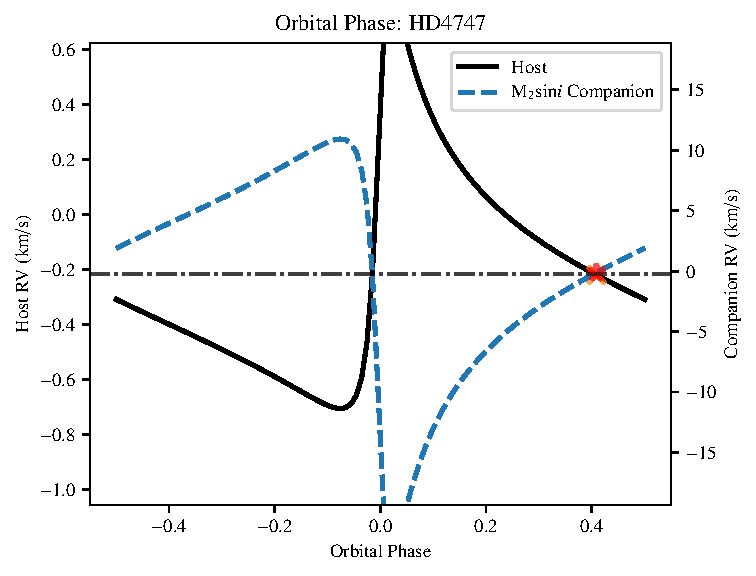
\includegraphics[width=0.45\linewidth]{figures/direct-recovery/orbital-plots/HD4747_orbital_phase.pdf}& 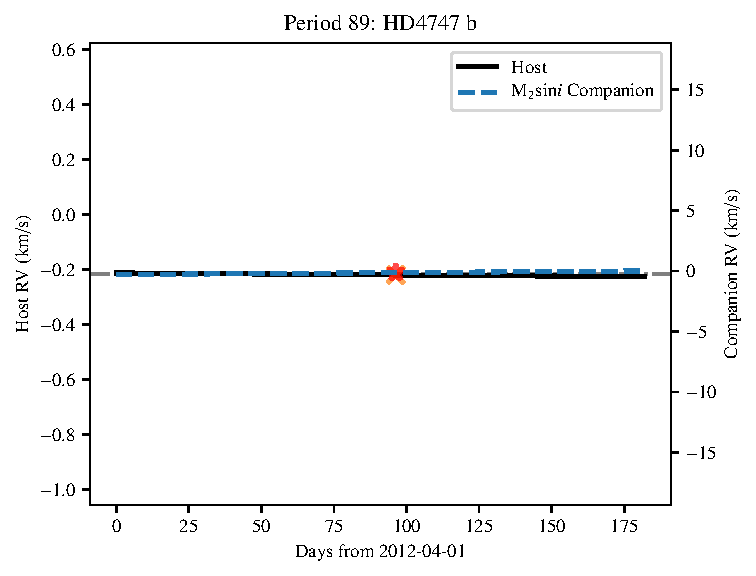
\includegraphics[width=0.45\linewidth]{figures/direct-recovery/orbital-plots/HD4747_p89.pdf}\\
    \end{tabular}
    \caption{RV orbital single companion Keplerian for the {HD\,4747}.
The left hand plot shows the RV curve for one full orbit while the right hand panel shows the RV curve over 6 months (Period 89).
The solid black line indicates the RV of the host star (with scale on the left), while the blue dashed line indicates the RV of the companion (with scale on the right axis).
The orange crosses and red stars indicate the times at which observations were obtained for the target, for the host and companion respectively.}
    \label{fig:hd4747p89}
\end{figure}

\begin{figure}
    \centering
    \begin{tabular}{cc}
        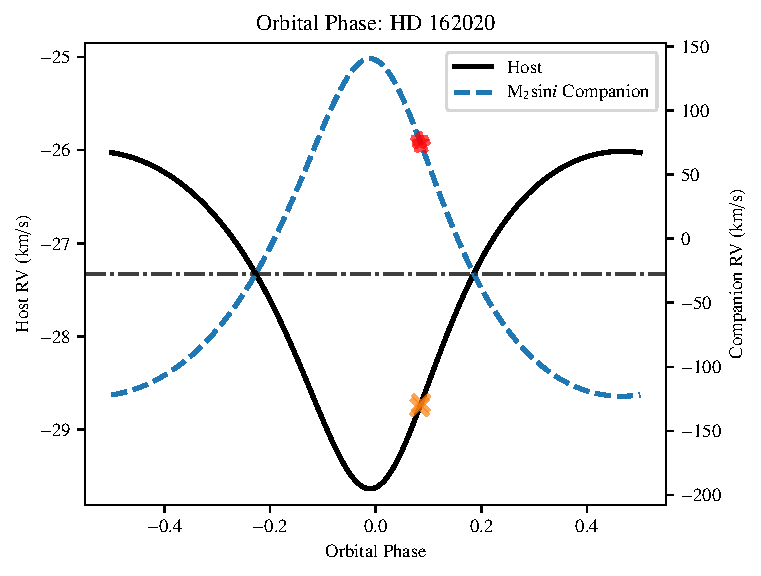
\includegraphics[width=0.45\linewidth]{figures/direct-recovery/orbital-plots/HD162020_orbital_phase.pdf}&
        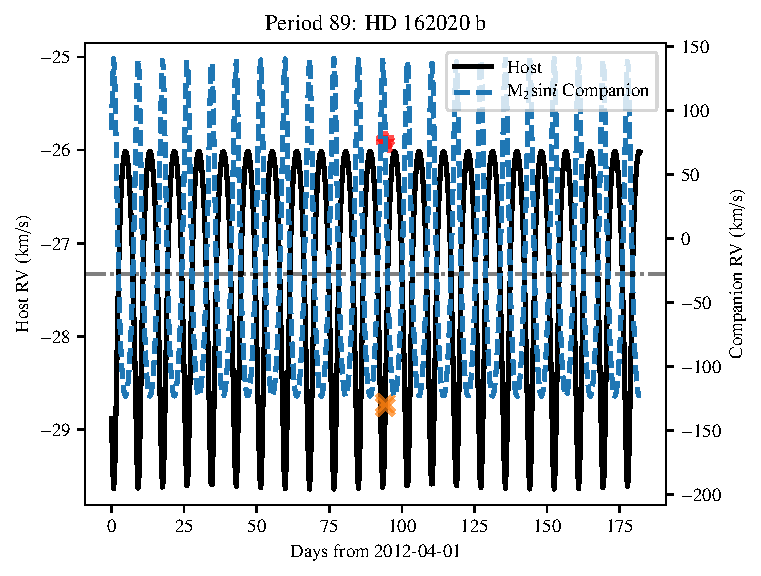
\includegraphics[width=0.45\linewidth]{figures/direct-recovery/orbital-plots/HD162020_p89.pdf}\\
    \end{tabular}
    \caption{Same as \fref{fig:hd4747p89} but for {HD\,162020}.}
    \label{fig:hd162020p89}
\end{figure}

\begin{figure}
    \centering
    \begin{tabular}{cc}
        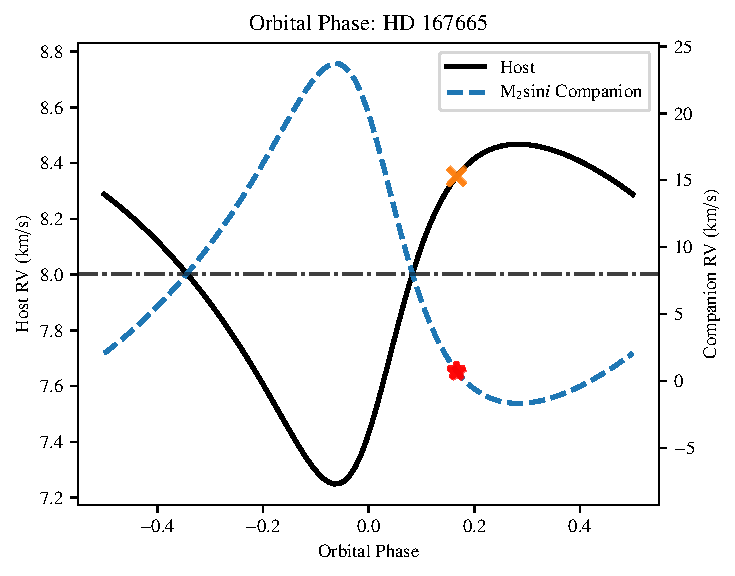
\includegraphics[width=0.45\linewidth]{figures/direct-recovery/orbital-plots/HD167665_orbital_phase.pdf}&
        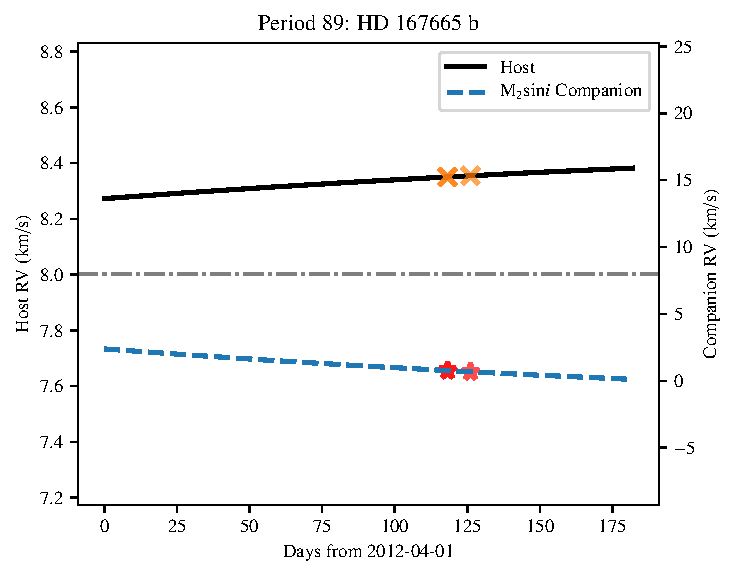
\includegraphics[width=0.45\linewidth]{figures/direct-recovery/orbital-plots/HD167665_p89.pdf}\\
    \end{tabular}
    \caption{Same as \fref{fig:hd4747p89} but for {HD\,167665}.}
    \label{fig:hd167665p89}
\end{figure}

\begin{figure}
    \centering
    \begin{tabular}{cc}
        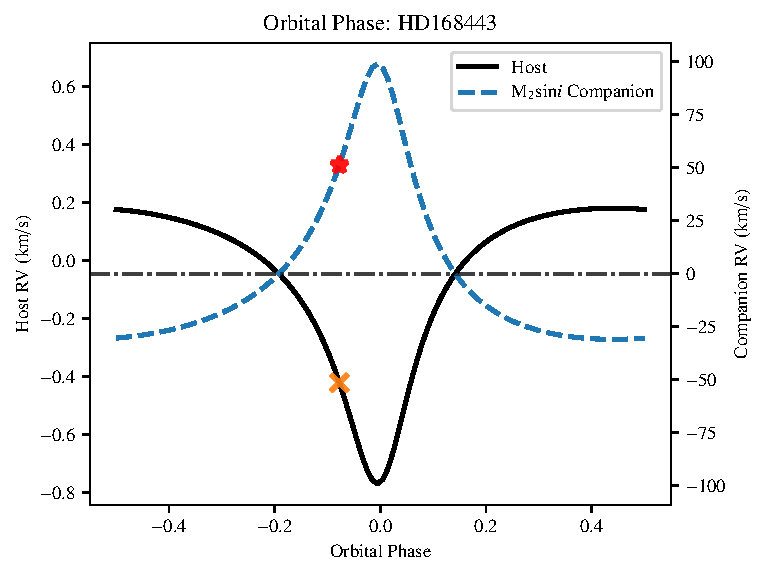
\includegraphics[width=0.45\linewidth]{figures/direct-recovery/orbital-plots/HD168443b_orbital_phase.pdf}&
        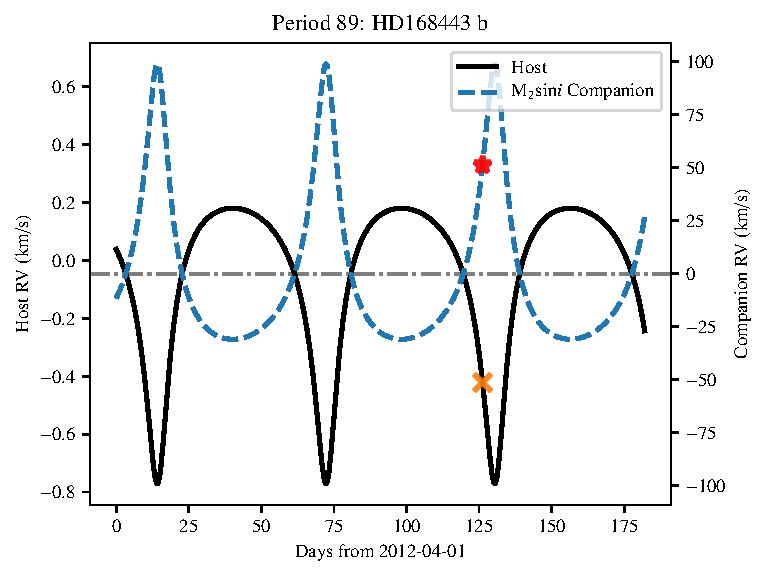
\includegraphics[width=0.45\linewidth]{figures/direct-recovery/orbital-plots/HD168443b_p89.pdf}\\
    \end{tabular}
    \caption{Same as \fref{fig:hd4747p89} but for {HD\,168443}b.
    Analysed as if this was a single companion.}
    \label{fig:hd168443bp89}
\end{figure}


\begin{figure}
    \centering
    \begin{tabular}{cc}
        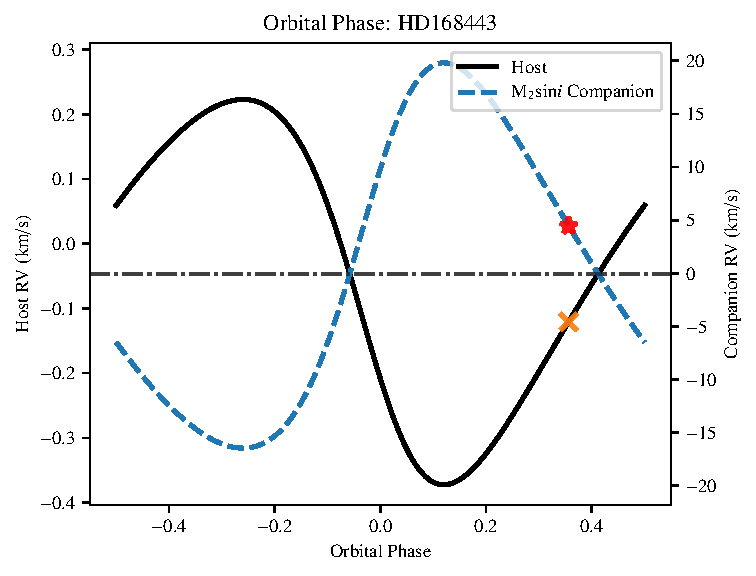
\includegraphics[width=0.45\linewidth]{figures/direct-recovery/orbital-plots/HD168443c_orbital_phase.pdf}&
        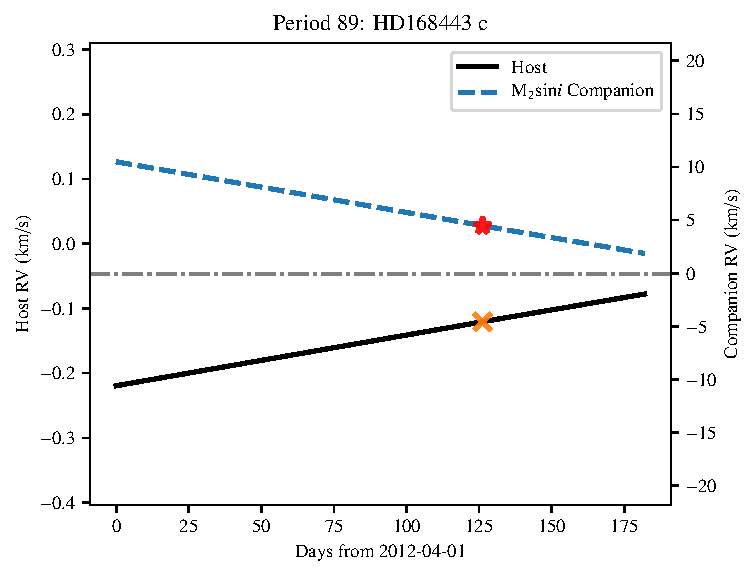
\includegraphics[width=0.45\linewidth]{figures/direct-recovery/orbital-plots/HD168443c_p89.pdf}\\
    \end{tabular}
    \caption{Same as \fref{fig:hd4747p89} but for {HD\,168443}c.
Analysed as if this was a single companion.}
    \label{fig:hd168443cp89}
\end{figure}

\begin{figure}
    \centering
    \begin{tabular}{cc}
        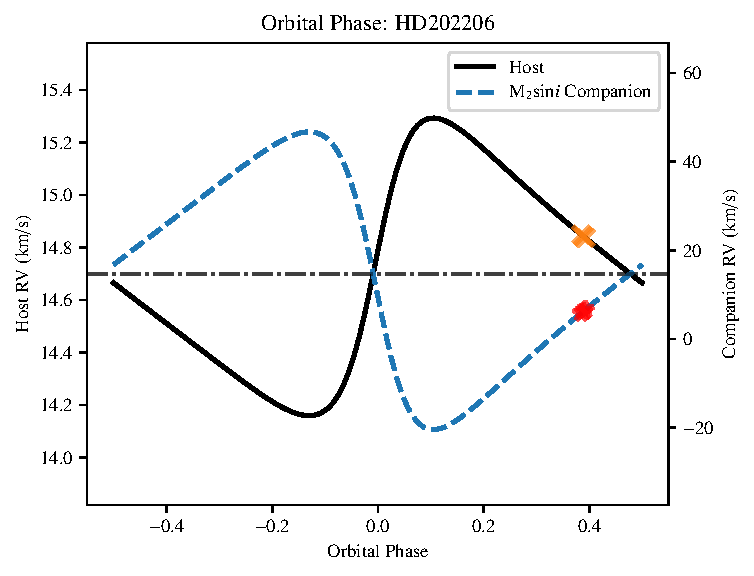
\includegraphics[width=0.45\linewidth]{figures/direct-recovery/orbital-plots/HD202206B_orbital_phase.pdf}&
        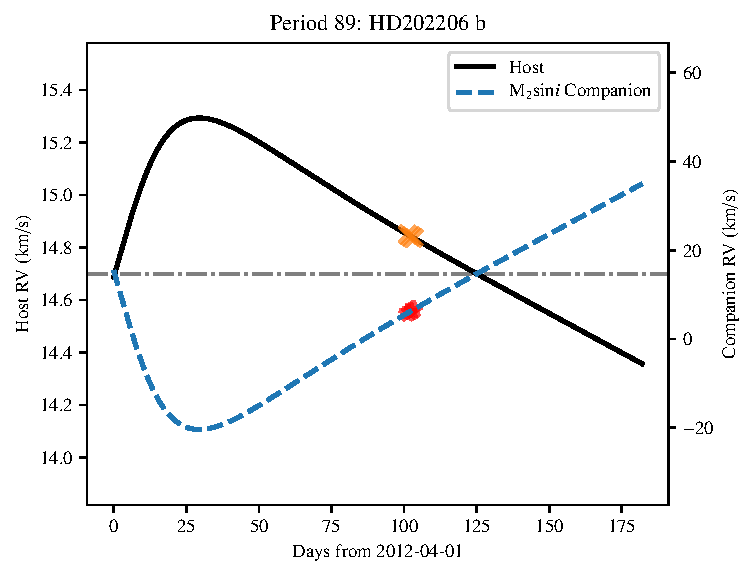
\includegraphics[width=0.45\linewidth]{figures/direct-recovery/orbital-plots/HD202206B_p89.pdf}\\
    \end{tabular}
    \caption{Same as \fref{fig:hd4747p89} but for {HD\,202206}B.
Analysed as if this was a single companion.}
    \label{fig:hd202206bp89}
\end{figure}

\begin{figure}
    \centering
    \begin{tabular}{cc}
        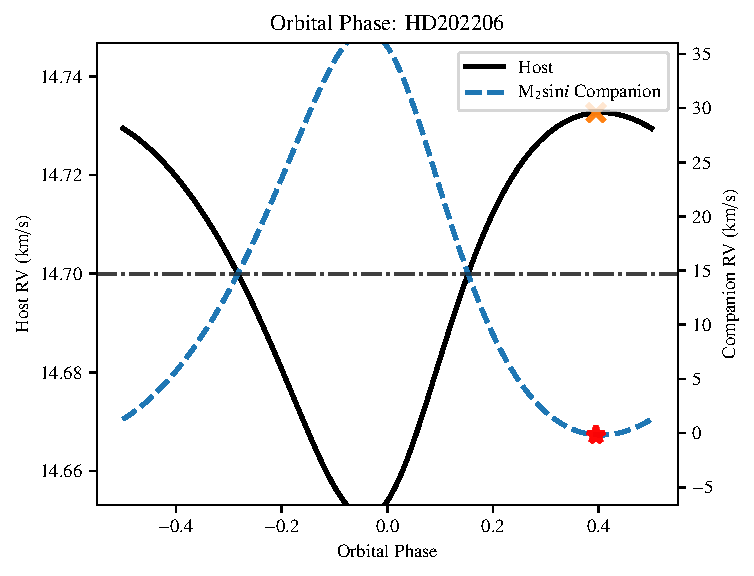
\includegraphics[width=0.45\linewidth]{figures/direct-recovery/orbital-plots/HD202206c_orbital_phase.pdf}&
        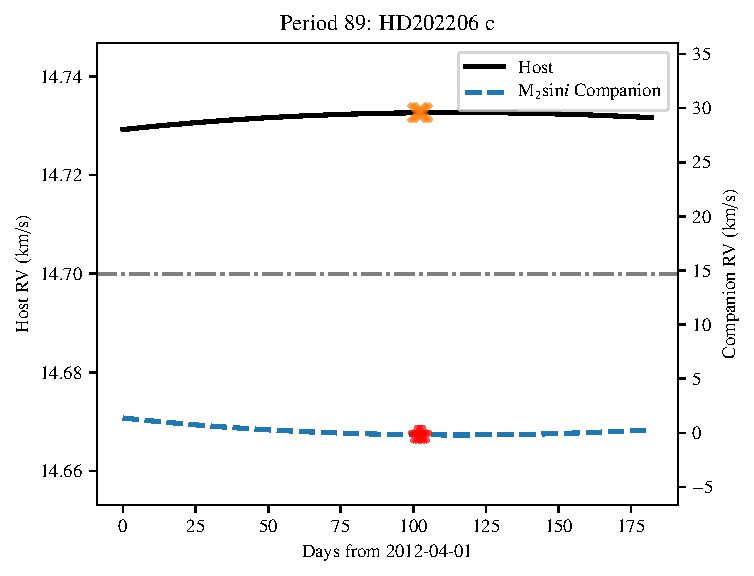
\includegraphics[width=0.45\linewidth]{figures/direct-recovery/orbital-plots/HD202206c_p89.pdf}\\
    \end{tabular}
    \caption{Same as \fref{fig:hd4747p89} but for {HD\,202206}c.
Analysed as if this was a single companion. }
    \label{fig:hd202206cp89}
\end{figure}

\begin{figure}
    \centering
    \begin{tabular}{cc}
        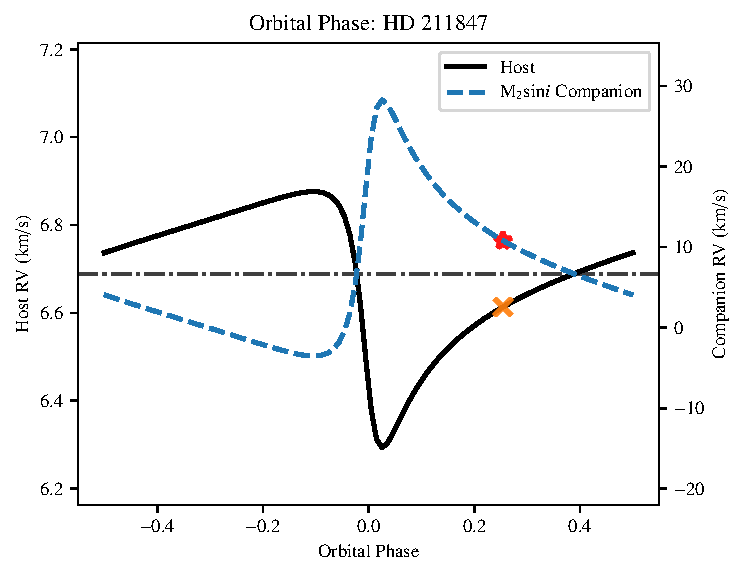
\includegraphics[width=0.45\linewidth]{figures/direct-recovery/orbital-plots/HD211847_orbital_phase.pdf}&
        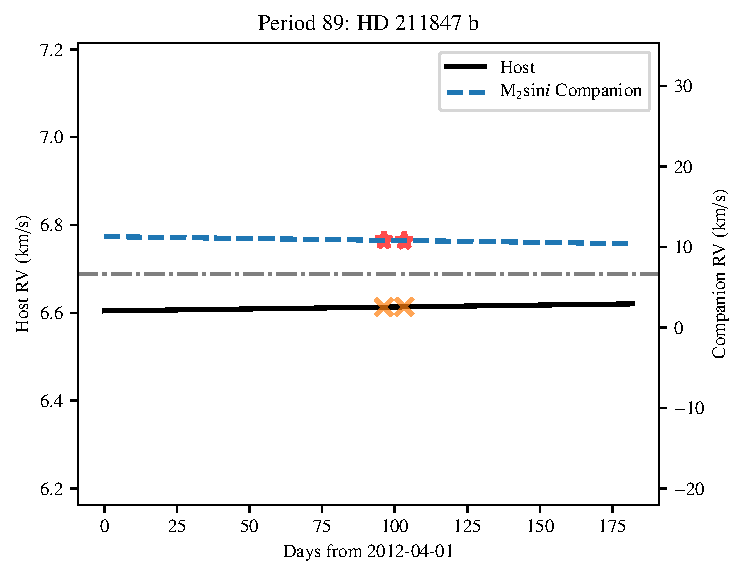
\includegraphics[width=0.45\linewidth]{figures/direct-recovery/orbital-plots/HD211847_p89.pdf}\\
    \end{tabular}
    \caption{Same as \fref{fig:hd4747p89} but for {HD\,211847}.}
    \label{fig:hd211847p89}
\end{figure}

\begin{figure}
    \centering
    \begin{tabular}{cc}
        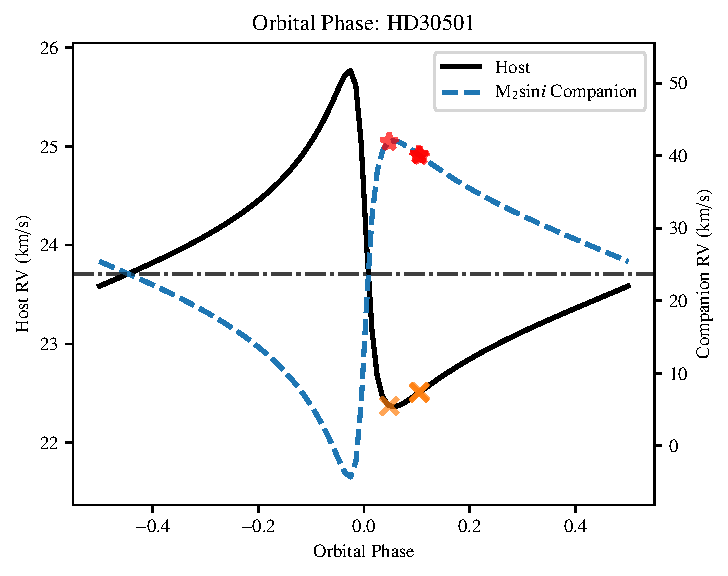
\includegraphics[width=0.45\linewidth]{figures/direct-recovery/orbital-plots/HD30501_orbital_phase.pdf}&
        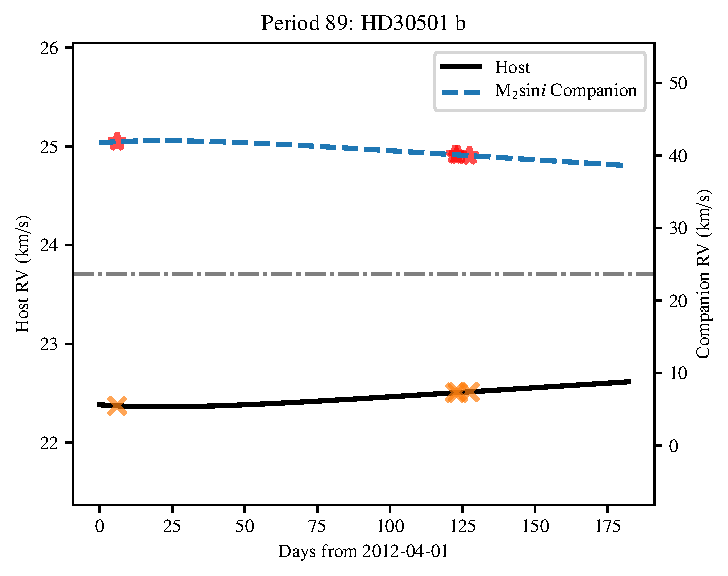
\includegraphics[width=0.45\linewidth]{figures/direct-recovery/orbital-plots/HD30501_p89.pdf}\\
    \end{tabular}
    \caption{Same as \fref{fig:hd4747p89} but for {HD\,30501}.}
    \label{fig:hd30501p89}
\end{figure}

\todo{Check M2sini labels - can we get M2 only for those that we know}

\todo{Should RV of companion be scale by m2sini only or m2 if known?}



\subsection{Relative differential amplitude}
To investigate the differential subtraction under tiny \(\Delta RV\), the change in differential amplitude against variation in {RV} was explored.
Simulations were performed creating a differential spectra for a range of \(\Delta {RV}\)s between \(\pm10\)\kmps{} using the same {PHOENIX-ACES} spectra for the companion of {HD\,30501} (\(\teff{}=2\,500\)\K{}, \logg{}=5.0, \feh{}=0.0) convolved to \(\R=50\,000\).
These simulations were focus on the wavelength range 2\,110--2\,123\nm{}, corresponding to detector \#1 of the {CRIRES} observations.
The differential spectra was created for each by taking the synthetic spectrum for the companion, Doppler shifting a copy of the spectrum and subtracting it from the original.
At each {RV} step the maximum absolute differential amplitude (peak to peak) of the simulated differential spectrum observed was recorded.
Again these simulations are performed assuming perfect telluric correction and removal of the host star by only considering the spectrum of the companion alone.

The result of this simulation is given in \cref{fig:diff_amp}.
As this absolute amplitude is specific to the lines present in the analysed wavelength range, the values were normalized by the median amplitude value outside of the line {\fwhm} (dashed vertical lines), between \(\pm(7-10)\)\kmps{}, to give a relative differential amplitude, independent from the depth of a specific line.
Differential subtraction simulations we also performed using a spectrum made up of a single Gaussian line and a single Lorentzian; these are shown in \cref{fig:diff_amp} as the orange dashed and green dash-dotted lines respectively.
The spectral profile shape of differential for the Gaussian line was also checked for consistency with the analytical form of the differential spectra from~\citet[][Equation~A.1]{ferluga_separating_1997} (included above as \cref{eqn:sprofile_gaussain}).

\cref{fig:diff_amp} shows that with a \(\Delta {RV}\) of zero between companion spectra the spectral lines of the companion completely cancel each other out, resulting in zero amplitude.
As the {RV} separation increases in either direction, the individual lines begin separating, and stop cancelling themselves out.
A maximum differential amplitude is achieved when the individual lines are fully separated.
We did not consider the shape/width of the differential spectral lobes as done in~\citet[][eqn.~A.1]{ferluga_separating_1997}, but this could also have been measured.

In the simulations of the synthetic spectrum (and of course real spectra) neighbouring spectral lines begin to strongly interfere, leading to a variable measured relative amplitude beyond 10 km/s.
The shape of the relative amplitude becomes complicated due to the interaction but since the \(\Delta {RV}\) for all the observations fall well short of this region it was not investigated further.
It is suspected that the interaction of neighbouring lines is one possible cause for the difference in the relative differential amplitude between the single theoretical line profiles and synthetic spectrum between 2 and 6\kmps{}.

The vertical dotted lines indicate the line \(\rm {\fwhm} = \lambda /\R=v /c \)velocity of 6\kmps{} at 2\um{} with \R=50\,000, showing that the amplitude is almost maximum when the lines are separated beyond their line width.
The two solid vertical lines in \cref{fig:diff_amp} indicate the \(\Delta \textrm{RV}\)=1.41\kmps{} separation calculated for our best target, {HD\,30501} from \cref{tab:estimated_rv}, given known orbital parameters and the observation times.
This shows that our differentials have severely reduced amplitude, \(<20\%\) relative to well separated individual lines.
As the companion spectra are already faint and in combination with a host star at >1\% flux ratio the >80\% extra reduction in signal amplitude makes this detection impossible with these observations.

\begin{figure}
    \centering
    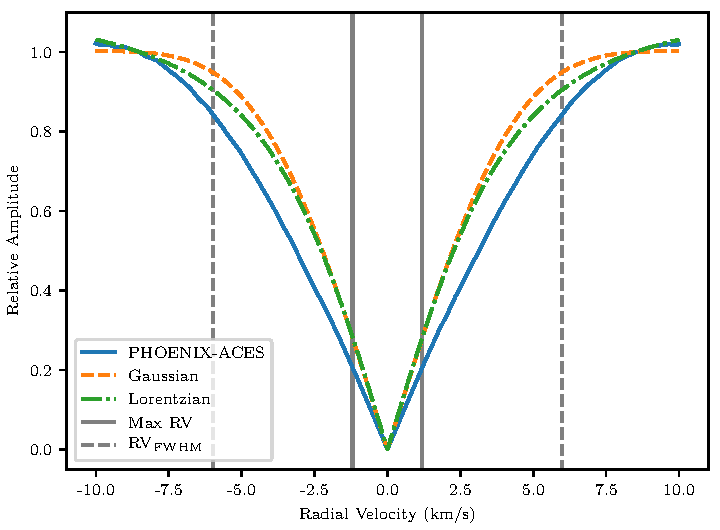
\includegraphics[width=0.8\textwidth]{figures/direct-recovery/rv_diff_final.pdf}
    \caption{Simulated relative amplitude of differential spectra at different companion \(\Delta RV\) separations revealing the diminished amplitude at very small orbital separations.
    The solid blue line shows the maximum relative amplitude of the differential signal (from a shifted copy of itself) of a {PHOENIX-ACES} spectrum with \(\teff{}=2500\)\K{}, \logg{}=5.0, \feh{}=0.0 in the wavelength region 2\,110--2\,123\nm{}.
    The maximum difference is normalized by the median amplitude between \(\pm7\)--10\kmps{}, representing a complete line separation.
    The orange (dashed) and green (dot-dashed) lines represent the relative amplitude of a spectrum differential for a spectrum containing a single Gaussian or Lorentzian absorption line respectively, each with a unitary amplitude and a \(\rm {\fwhm} = \lambda / R\).
    The solid vertical lines indicate the estimated companion \(\Delta {RV}\) in these observations while the dashed vertical lines indicate the {RV} corresponding to the {\fwhm} at this wavelength and resolution.}
    \label{fig:diff_amp}
\end{figure}
\unfinished{Increase size of diff amp plots to two}








\subsubsection{Differential scheduling challenges {copy from paper}}
\label{subsubsec:differential-schedualing}
This work has revealed that more care needs to be taken in planning the observations for the spectral differential analysis of faint companions in the future.
Paying attention in particular to the {\fwhm} of the lines in the region (governed by resolution and wavelength); the estimated companion \(\Delta {RV}\); the previous observations from different observing periods; and keeping consistent detector settings.

The original goal for the observations was to obtain two different and ``clearly separated radial-velocities'' for the secondary companion.
However, the program was assigned a low-priority (C, in ESO grading) and, possibly due to operational reasons, the original time requirements necessary to secure well separated RVs for the companion spectra could not be met.
This meant that all observations were insufficiently separated to extract a differential spectra for the companion.

The long orbital periods of these targets is also a contributing factor to the insufficient separations.
Most of the targets observed here have orbital periods much longer than an observing semester (183 days).
An optimal pair of observations (achieved at the extrema) would need to have been obtained from separate observing periods (between 2 months and 19 years apart).
In some cases, even observations taken at the beginning and end of a single observing semester would not be sufficient to achieve companion separation (depending on the phase), requiring separate observing periods to even achieve the minimum \(\Delta \rm {RV}\) larger than the line {\fwhm}.
At the time it was impossible to ask for time over several semesters in a regular proposal.

This study demonstrates the importance of proposals for projects that need to be extended over several semesters or years.
In the ESO context, this corresponds to ``Monitoring proposals''~\citep[e.g.][pg.~18]{eso_eso_2017}.
Observations of the targets explored here, with long orbital periods in particular, would benefit from the ability for multi-period proposals and newer scheduling systems which allow for tighter scheduling constraints, such as a companion {RV} separation.

For future observations we suggest that the known orbital solution of the companion be used to estimate the companions' {RV} curve during the observing period, with the companion \Mtwosini{} providing an {RV} upper-limit.
Knowing the instrumental wavelength and resolution, a constraint can then be set to avoid taking observations when the companion spectra are insufficiently separated, or \(\Delta {RV}\) < {\fwhm}.
This constraint can be set using the absolute and relative \emph{time-link} constraints available in {ESO}'s {Phase 2 Proposal Preparation} (P2PP) tool.
Additionally, analysing the known orbital solution beforehand to determine {RV} constraints will also help identify the best time to observe, if observations from separate periods will be required or, if an optimally separated companion differential is even feasible.
Again the phase 2 proposal documentation for these observations could not be obtained to check if these observations had used any of these features, which were available at the time.





\textbf{
CHECK out LOCKWOOD 2014 - maximum likelihood with todcor 1e-4 flux ratio double lined spectra}




\section{Direct recovery in the \mir{}}
It was investigated if this differential technique could be extended into the mid-infrared {\mir{}} domain.
There were two reasons for this: to develop experience with the {\mir{}} domain where the contrast ratios are higher, and due to the lack of high-resolution \nir{} spectrographs available at the time (see \cref{subsec:new_generation}).

{VISIR} is a \mir{} spectrograph on the {VLT}, offering diffraction-limited imaging at high sensitivity in three mid-infrared (\mir) atmospheric windows: the \emph{M}-band at 5\um{}, the \emph{N}-band between 8--13\um{} and the \emph{Q}-band between 17--20\um{}, respectively.
The use of {VISIR} to detect the spectra of Brown Dwarf companions in the {\mir{}} was briefly explored.
The candidate selected as the best target to investigate was {HD\,219828} which has a hot-Neptune (\Mtwosini{}=21\Mearth)~\citep{melo_new_2007} and a recently discovered super Jupiter (\Mtwosini{}=15.1\,\Mjup) on a long period (13 yr) eccentric orbit (e=0.81)\citep{santos_extreme_2016}.

Based on the spectra of a cool brown dwarfs in the \mir{}, and the detector configuration available at the time, the best option for the observations was the low resolution mode covering the wavelength region 8--13\um{}.
This wavelength region would have encompassed the \ce{NH4} signature at 10.5\um{} and the edge of a \ce{CH4} band at 7.7\um{}, both large features in the BD \mir{} spectrum.

After performing flux ratio calculations between the host and companion using the~\citet{baraffe_evolutionary_2003} models (see \cref{subsec:compaion_flux_ratio}) and considering the performance of the {VISIR} instrument and the exposure time calculator it was determined that observations with {VISIR} to achieve a \snr{} of 100 were infeasible, requiring 1\,000's of hours of observing time to achieve the necessary signal-to-noise level to separate the companion from a blended spectra.
As such the direct separation approach was not continued further in the \mir{}.



...

\textbf{This method is very similar to~\citet{kostogryz_spectral_2013} except that they focus on M-dwarfs host stars with the observations taken at the extrema, in which the companion lines are well separated. \todo{They get a result???}
}
\section{Summary}
This Chapter presented the observations that were gathered having in mind the application of a differential subtraction method~\citep[e.g.][]{ferluga_separating_1997, kostogryz_spectral_2013} to recover the spectra of the faint {BD} companions.  Due to the poorly separated observation times relative to the long orbital periods, the differential subtraction method presented in \cref{sec:direct-subtraction} was revealed to be inappropriate for these observations as the {RV} separation of the companion spectra between observations is significantly smaller than the width of individual spectral lines.
The small separation of the companion causes the lines of the companion to also mutually cancel, severely reducing the residual signal to well below the available noise level.
The requirement of well separated RVs for the companion spectra was clearly stated in the original proposal but was not satisfied by the observations. {\red{} The very large orbital periods of some of the targets would not produce a sufficient {RV} signal during one semester.
This was a possible oversight during the proposal stage.} The largest estimated companion \(\Delta {RV}\) separation between the observations of each target is provided in the  \nth{7} column of \cref{tab:estimated_rv}. \todo{move}{Radial velocity constraints are also valid for other studies such as the detection of reflected light from exoplanets~\cite[e.g.]{martins_evidence_2015}.}
